\documentclass[12pt]{article}
\usepackage[letterpaper]{geometry}
\geometry{top=1.0in, bottom=1.0in, left=1.0in, right=1.0in}
\usepackage{graphicx}
\graphicspath{{images/}}

\begin{document}

\begin{flushright}
Jean-Ralph Aviles\\
EEL 3744\\
Section 1539\\
Lab 0 Prelab\\
\end{flushright}

\section{Questions}
\begin{enumerate}
\item What minimum lab average is required in order to be
eligible to pass the course? \\
\hspace*{4ex} According to the syllabus, a lab grade of 65\% or higher is required to obtain a passing grade.
\item How late can you arrive for lab and still be admitted? How late can you arrive for lab and still be allowed to take the lab quiz? \\
\hspace*{4ex} You can arrive up to 30 minutes late for lab, but you will be at the bottom of the TA's priority list. You can only take the lab quiz if you are less then 10 minutes late.
\item When soldering a wire to a pin, what should the
soldering iron touch and what should the un-melted
solder touch?\\
\hspace*{4ex} The soldering iron should touch both the pad on the PCB and the component lead coming up through the board. The solder should feed in from the side opposite the iron and touch the component coming up.
\item What is the lab makeup policy if you miss a single
lab? Can you drop this lab if ... a) you overslept? b)
project for other class due? \\
\hspace*{4ex} The makeup policy for labs is as follows. You can miss one lab for free, with no penalty or having to show a proper excuse, but if you miss your second lab you must show documentation for both the first lab and second labs. So if you overslept one time you better not miss another lab.
\item How many turns of bare wire should be on a wire wrap pin? How much wire (in inches) do you need to strip to get these turns on the pins? How many wraps of insulation should be on a wire wrap pin? \\
\hspace*{4ex} There should be 5-7 turns of bare wire on the pin. To get these turns in you need about 1 inch of bare wire stripped plus a little bit extra for the 1-1.5 wraps of insulated wire on the pin.
\end{enumerate}

\section{Problems Encountered}
\begin{enumerate}
\item Had to install Windows 10 under VirtualBox because Atmel Studio is not supported for OSX.
\end{enumerate}
\section{Future Work/Applications}
\begin{enumerate}
\item Wire wrapping is useful for tinkering with electronics without having to use a soldering iron. If you are ever in an area where soldering irons are not available, then this an option.
\end{enumerate}

\section{Appendix}
\begin{enumerate}

\item Atmel Studio Screenshot for the Prelab Requirements
\begin{center}
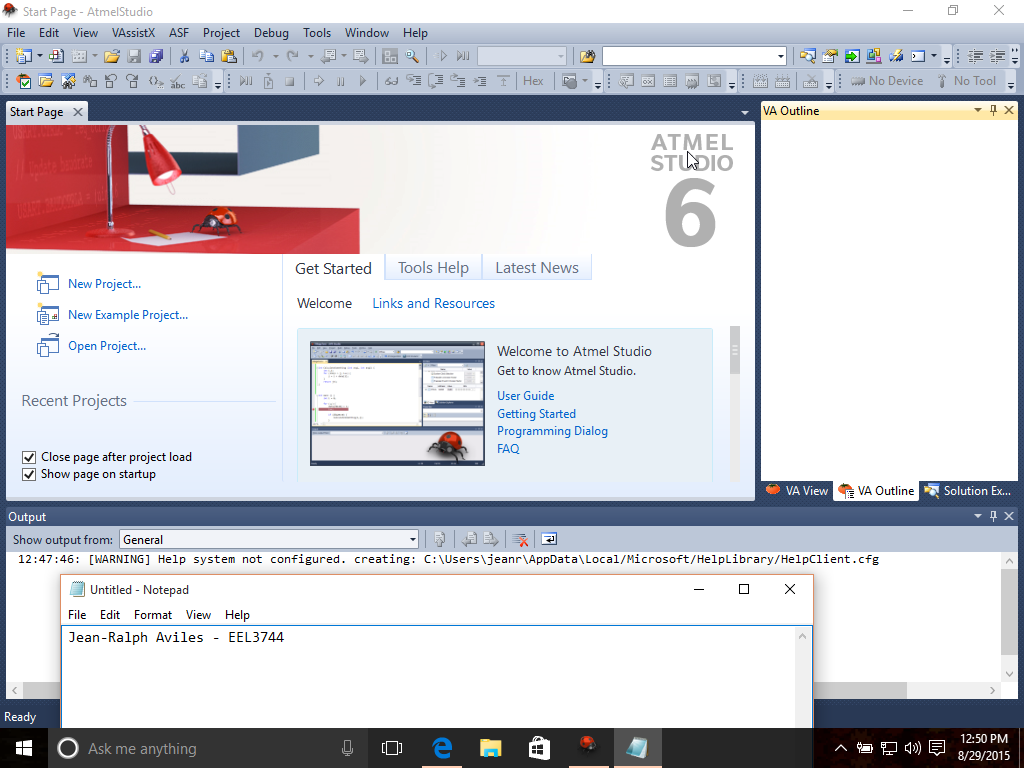
\includegraphics[width=\textwidth]{atmel}
\end{center}

\end{enumerate}

\end{document}